\chapter{Resultados}
\label{chap:resultados}

\section{Clock}
O clcck foi implementado para contar 1 segundo, e ele é utilizado para a fazer a contagem do tempo de ativação da armadilha e para a geracao do numero aleatório.

\begin{figure}[H]
    \centering
    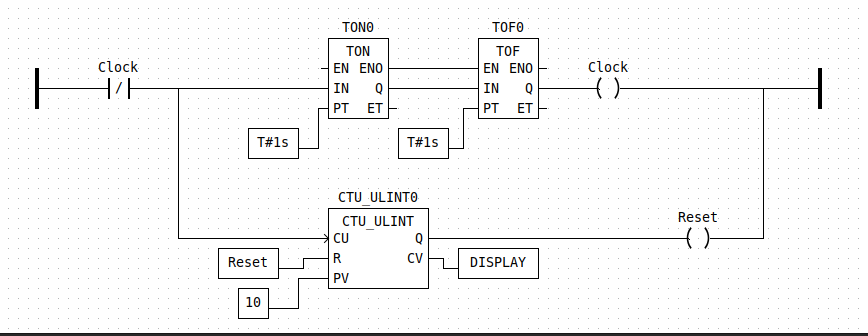
\includegraphics[width=0.8\textwidth]{images/clock.png}
    \caption{Clock}
    \label{fig:clock}
\end{figure}

\section{Extrator de Digitos}
O extrator de digitos foi implementado para separar os digitos do numero aleatório gerado, para que cada digito possa ser comparado com o botao pressionado pela vitima.

\begin{figure}[H]
    \centering
    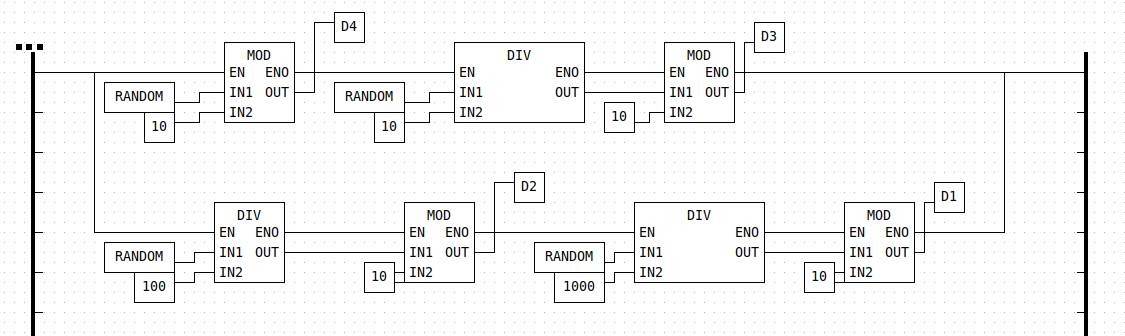
\includegraphics[width=0.8\textwidth]{images/digit_extractor.png}
    \caption{Extrator de Digitos}
    \label{fig:extrator_de_digitos}
\end{figure}

\section{Gerador de Numero Aleatório}
Para se gerar o numero aleatorio utilizou-se do Hull-Dobell Linear Congruential Generator definido por:

\begin{equation}
X_{(n+1)} = (aX_n + c)mod m
\end{equation}

Onde:
\begin{itemize} 
  \item m > 0
  \item 0 < a < m
  \item 0 <= c < m
  \item 0 <= X < m
  \item m potencia de 2, aki $ m = 2^{32} $
  \item a-1 divisivel por todos fatores primos de m, ou seja apenas divisivel por 2
  \item c diferente de 0
  \item m e c sao coprimos, c impar entao automaticamente coprimo de m
\end{itemize}

Para esse LCG utilizou-se os seguintes valores:
\begin{equation}
   a = 32310901
   c = 32310901
   m = 4294967296
\end{equation}

Deve gerar um Random quando a armadilha for ativada pela primeira vez e sempre que a Vitima cometer um erro. Como O perido aki seria de m, tira-se o modulo por 10000 para ter-se numeros entre 0-9999

\begin{figure}[H]
    \centering
    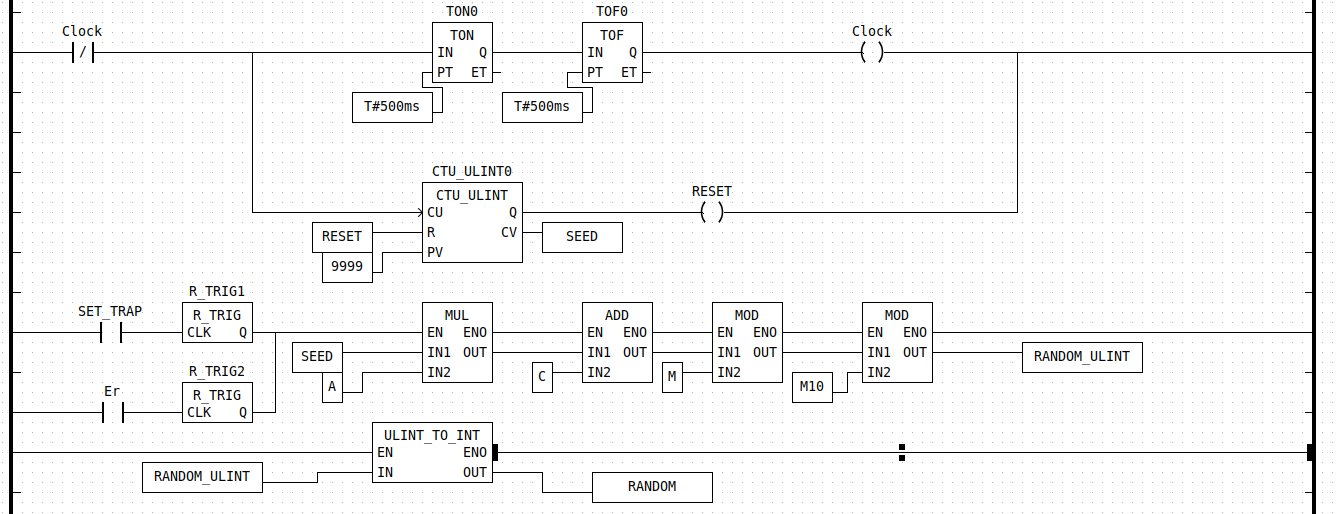
\includegraphics[width=0.8\textwidth]{images/random_generator.png}
    \caption{Gerador de Numero Aleatório}
    \label{fig:gerador_de_numero_aleatorio}
\end{figure}

\section{Temporizador}
Toda Vez que um erro ocorre (Er) deve-se remover 10s do Temporizador. Note que o programa usa um cronometro para se chegar ao tempo inbutido atraves das variaveis de entrada para minutos e segundos, porem o display exibe os valores como um temporizador. Para isso, o tempo total e convertido em um unico TIMER e depois manipulado para ser exibido como um temporizador.
A conversao para um TIMER total impede que se tenha valores negativos para segundos com a subtração por erro.
Ah mais não vai fica abaixo de zero quando ele erra os segundos forem menores que 10?
Não por que a conversao trabalha com o total em segundos e depois realizar a reconversao para minutos e segundos quand for exibir no display

\begin{figure}[H]
    \centering
    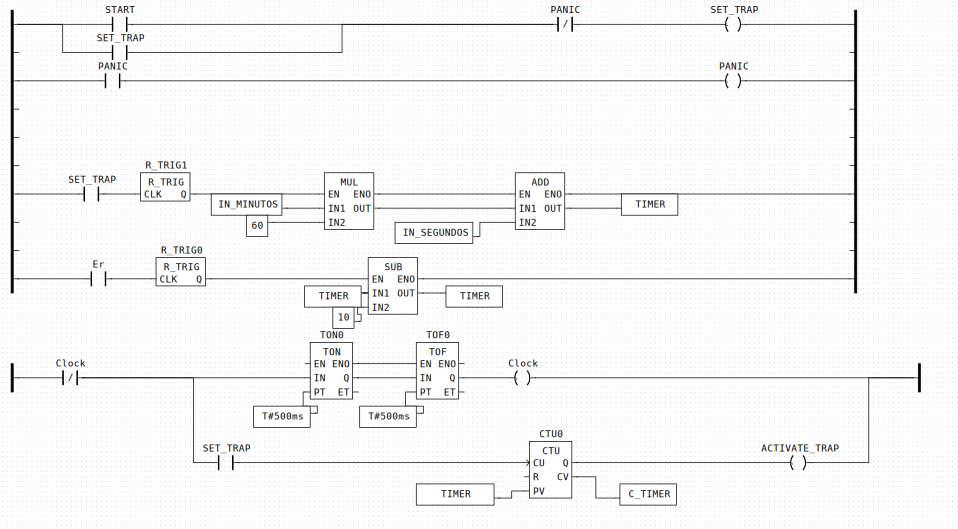
\includegraphics[width=0.8\textwidth]{images/sub_timer.png}
    \caption{Temporizador}
    \label{fig:temporizador}
\end{figure}

O Display converte o valor do TIMER, que é um cronometro, para o formato de um temporizador através de operações matematicas simples.

\begin{figure}[H]
    \centering
    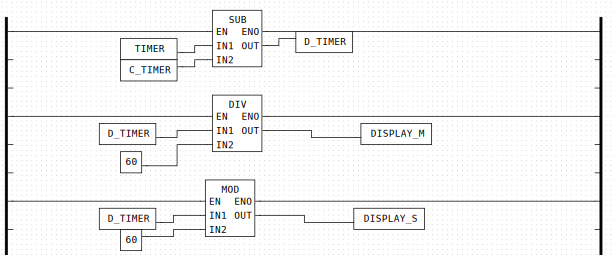
\includegraphics[width=0.8\textwidth]{images/display.png}
    \caption{Display do Temporizador}
    \label{fig:display_do_temporizador}
\end{figure}


\section{Botões}
Os botões são implementados como entradas digitais, e cada botão corresponde a um número de 1 a 4. Quando um botão é pressionado, o sistema verifica se o número do botão corresponde ao dígito atual do puzzle que a vítima deve pressionar. 
A seguinte imagem representa a implementação do botão 1, os outros botões são implementados de forma semelhante.

\begin{figure}[H]
    \centering
    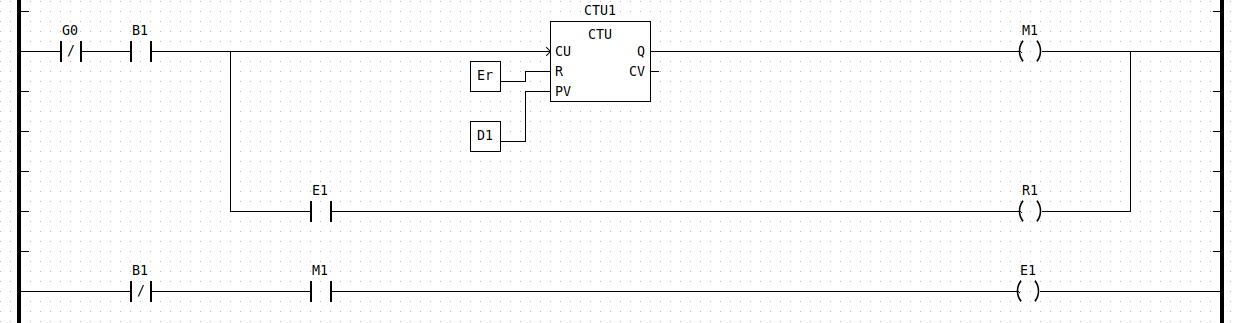
\includegraphics[width=0.8\textwidth]{images/button_input.png}
    \caption{Botão 1}
    \label{fig:botao_1}
\end{figure}

\subsection{Guarda de Pressionamento}
Guarda para garantir que não há mais de um botao sendo pressionado ao mesmo tempo
Usar combinacao de 4 em 2 = 6, de 4 em 3 = 4 e de 4 em 4 = 1 atraves da formula:
\begin{equation}
  c = \frac{n!}{r!(n-r)!}
\end{equation}

\begin{figure}[H]
    \centering
    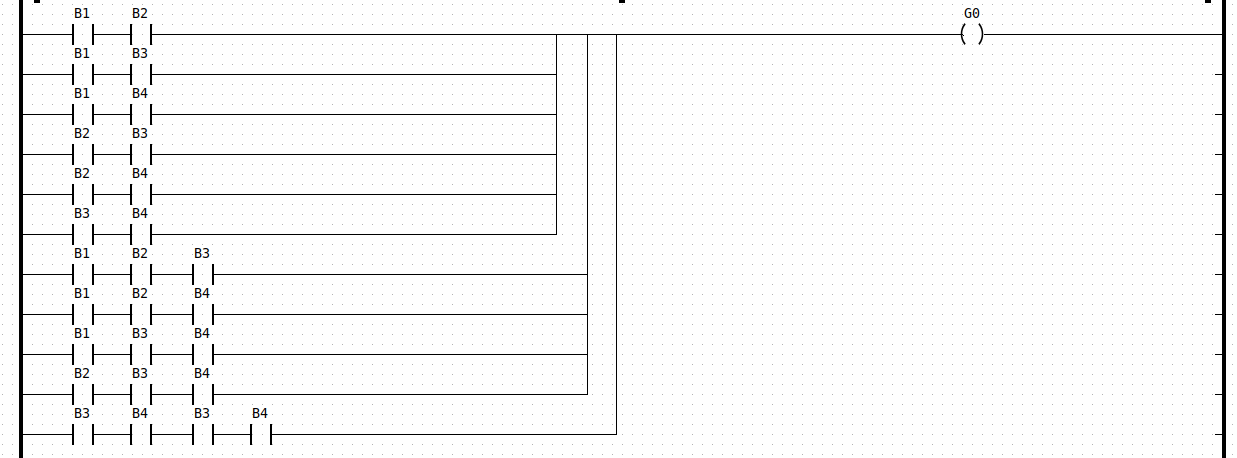
\includegraphics[width=0.8\textwidth]{images/button_guard.png}
    \caption{Guarda de Pressionamento}
    \label{fig:guarda_de_pressionamento}
\end{figure}

\subsection{Guarda de Valor}
Qualquer valor 0 em um dos digitos automaticamente ativa a memoria correspondente, independentemente da ordem. Por isso deve-se guardar a logica das outras memorias quand uma delas esta sempre ativa, não ativar erro de ordem quando uma delas é sempre positiva

\begin{figure}[H]
    \centering
    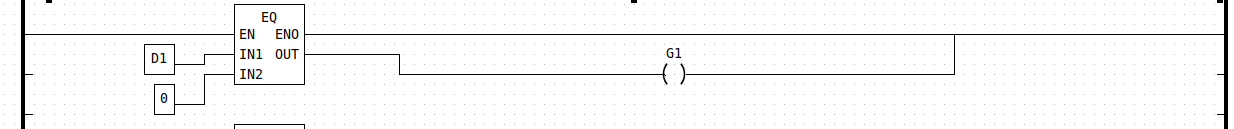
\includegraphics[width=0.8\textwidth]{images/button_value_guard.png}
    \caption{Guarda de Valor}
    \label{fig:guarda_de_valor}
\end{figure}

\subsection{Casos de Ordem}
A cada botao pressionado, deve-se verificar se o botao pressionado é o correto.

\begin{figure}[H]
    \centering
    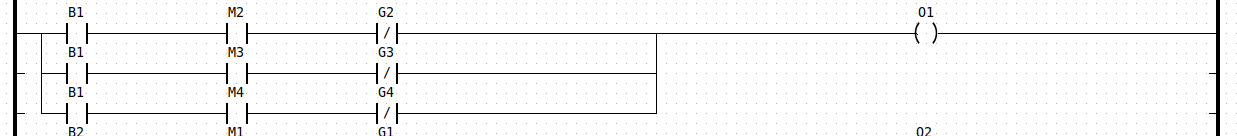
\includegraphics[width=0.8\textwidth]{images/button_order_case.png}
    \caption{Casos de Ordem}
    \label{fig:casos_de_ordem}
\end{figure}
